% ─────────────────────────────────────────────────────────────────────────────
% CHAPTER 6: Results and Interface Walkthrough
% ─────────────────────────────────────────────────────────────────────────────

This chapter presents the experimental and functional results obtained from testing the complete GroDealz platform. It provides a visual walkthrough of the functioning web application using screenshots captured from the live deployment, reports the test outcomes of the automated test suites, and evaluates system latency and multi-store cost savings.

\section{Interface Walkthrough and Screenshots}

The deployed web application was tested on a live staging environment on Render connected to a MongoDB Atlas cluster. The following screenshots demonstrate the core functionalities implemented in this project:

\subsection{GroDealz Home and Personalized Recommendations}

Figure~\ref{fig:screen_home} shows the main customer landing interface of GroDealz.

\begin{figure}[H]
\centering
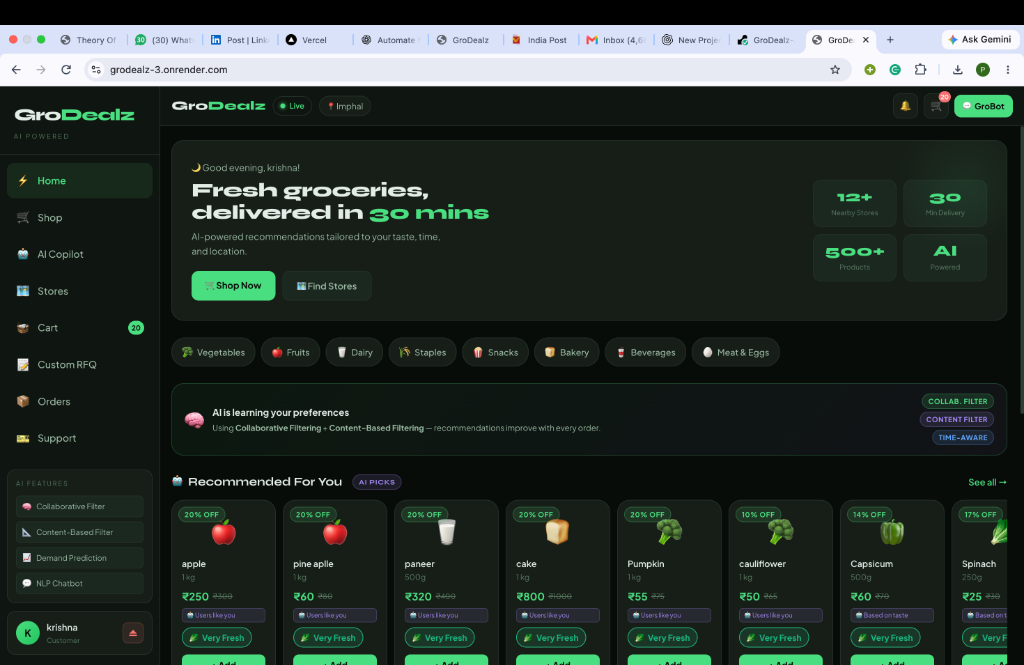
\includegraphics[width=0.96\textwidth,keepaspectratio]{figures/screenshot_home.png}
\caption{GroDealz Main Interface Featuring Personalized Recommendation Rails and Freshness Badges. Shows authenticated customer view, dynamic recommendation tags, categorized grocery items, and freshness confidence indicators.}
\label{fig:screen_home}
\end{figure}

Key functional elements visible on the screen include:
\begin{itemize}
    \item \textbf{Status and Platform Metrics:} Shows the live platform connection in Imphal, key performance highlights (12+ Nearby Stores, 30-minute delivery promise, 500+ fresh products, AI Powered), and active cart count.
    \item \textbf{AI Recommendation Banner:} The notification banner informs the user that the system combines collaborative filtering with content-based features, displaying the active tags: \texttt{COLLAB. FILTER}, \texttt{CONTENT FILTER}, and \texttt{TIME-AWARE}.
    \item \textbf{Category Navigation:} Quick-filter buttons allow switching between Vegetables, Fruits, Dairy, Staples, Snacks, Bakery, Beverages, and Meat \& Eggs.
    \item \textbf{Product Cards with Freshness Badges:} Each item displays its current price, discounted rate, user affinity indicator (e.g., \emph{``Users like you''} or \emph{``Based on taste''}), and a live confidence badge (\emph{``Very Fresh''}).
    \item \textbf{Sidebar Navigation:} Provides direct links to Home, Shop, AI Copilot, Stores, Cart, Custom RFQ, Orders, and Support, along with AI engine status pills.
\end{itemize}

\subsection{Autonomous AI Grocery Planner and Store Journey Audit}

Figure~\ref{fig:screen_ai_planner} illustrates the Autonomous Grocery Shopping Agent interface on \texttt{/ai-planner}.

\begin{figure}[H]
\centering
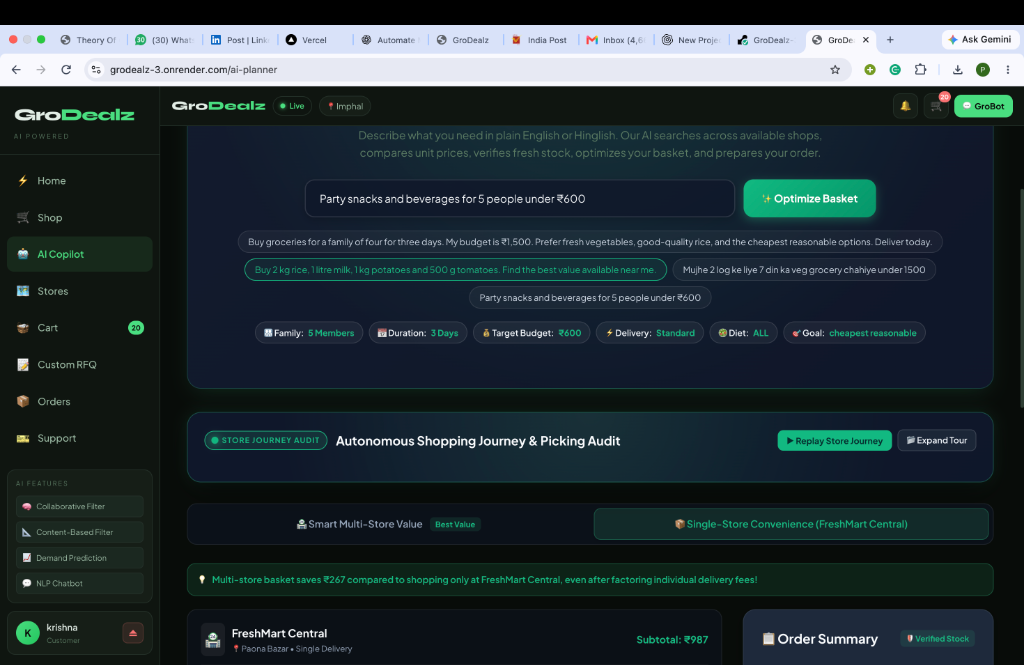
\includegraphics[width=0.96\textwidth,keepaspectratio]{figures/screenshot_ai_planner.png}
\caption{Autonomous Shopping Agent Interface with Store Journey Audit and Multi-Store Savings Proof. Illustrates natural language budget parsing, automated cross-store stock picking, and a calculated ₹267 net saving over single-store shopping.}
\label{fig:screen_ai_planner}
\end{figure}

The screenshot captures the complete execution flow of the autonomous agent:
\begin{itemize}
    \item \textbf{Natural Language Input:} The user entered: \emph{``Party snacks and beverages for 5 people under ₹600''}.
    \item \textbf{Extracted Parameter Chips:} The agent parsed the input into structured chips: \textbf{Family:} 5 Members, \textbf{Duration:} 3 Days, \textbf{Target Budget:} ₹600, \textbf{Delivery:} Standard, \textbf{Diet:} ALL, and \textbf{Goal:} cheapest reasonable.
    \item \textbf{Store Journey Audit:} The panel displays the \emph{``Autonomous Shopping Journey \& Picking Audit''} with interactive controls to replay the journey or expand the tour.
    \item \textbf{Smart Basket Comparison:} The system evaluates the multi-store split against single-store convenience (FreshMart Central).
    \item \textbf{Verified Net Savings Proof:} The green banner clearly proves the financial benefit to the customer: \emph{``Multi-store basket saves ₹267 compared to shopping only at FreshMart Central, even after factoring individual delivery fees!''}
\end{itemize}

\subsection{Custom Shopping Requirements and Reverse RFQ Marketplace}

Figure~\ref{fig:screen_buyer_rfq} shows the Customer RFQ screen (\texttt{/buyer-rfq}), which forms the foundation of Module~B.

\begin{figure}[H]
\centering
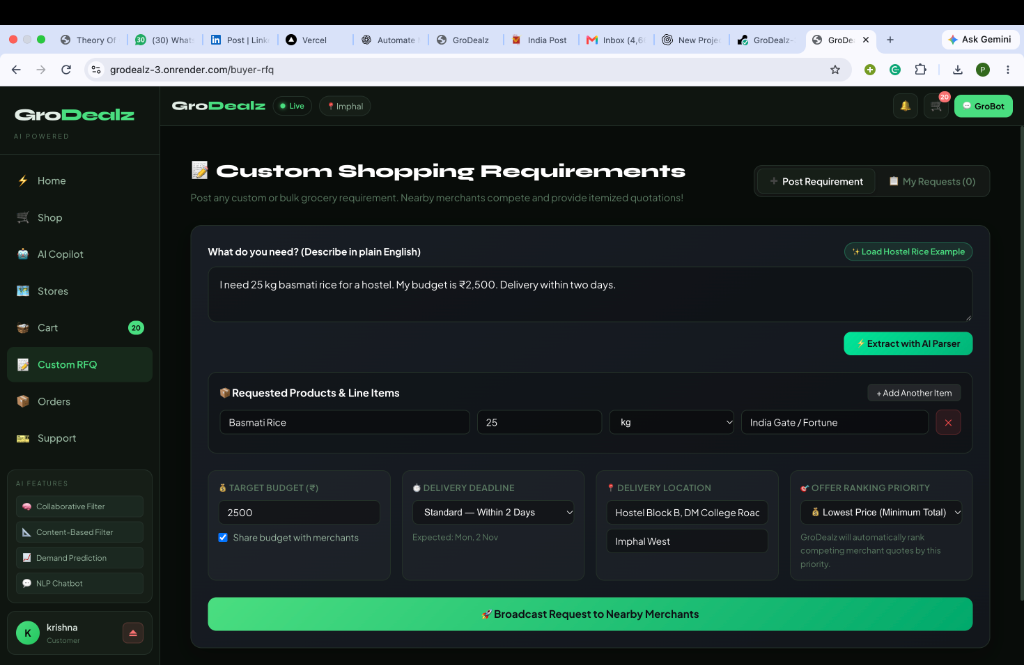
\includegraphics[width=0.96\textwidth,keepaspectratio]{figures/screenshot_buyer_rfq.png}
\caption{Customer Custom Shopping Requirements Interface with AI Line-Item Extractor and RFQ Controls. Demonstrates NLP parsing of bulk hostel rice requests, budget sharing toggles, ranking priority selectors, and instant merchant broadcast.}
\label{fig:screen_buyer_rfq}
\end{figure}

The screenshot illustrates:
\begin{itemize}
    \item \textbf{Requirement Input Box:} Displays the pre-filled hostel requirement: \emph{``I need 25 kg basmati rice for a hostel. My budget is ₹2,500. Delivery within two days.''}
    \item \textbf{AI Parser Extraction:} Clicking \emph{``Extract with AI Parser''} automatically extracted the commodity: \textbf{Basmati Rice}, Quantity: \textbf{25}, Unit: \textbf{kg}, and Preferred Brand: \textbf{India Gate / Fortune}.
    \item \textbf{Marketplace Parameters:} Shows the target budget set to ₹2,500 with the \emph{``Share budget with merchants''} checkbox enabled, the delivery deadline set to \emph{Standard --- Within 2 Days (Expected: Mon, 2 Nov)}, and the delivery location set to \emph{Hostel Block B, DM College Road, Imphal West}.
    \item \textbf{Offer Ranking Priority Selector:} Dropdown allows the customer to choose how competing quotations will be ranked: \textbf{Lowest Price (Minimum Total)}, \textbf{Fastest Delivery}, \textbf{Top Rated Merchants}, or \textbf{Balanced Composite}.
    \item \textbf{Broadcast Button:} The primary call-to-action (\emph{``Broadcast Request to Nearby Merchants''}) transmits the RFQ to nearby store dashboards in real time.
\end{itemize}

\subsection{AI Customer Support CRM and Ticket Triage}

Figure~\ref{fig:screen_support} shows the AI Customer Support interface (\texttt{/support}).

\begin{figure}[H]
\centering
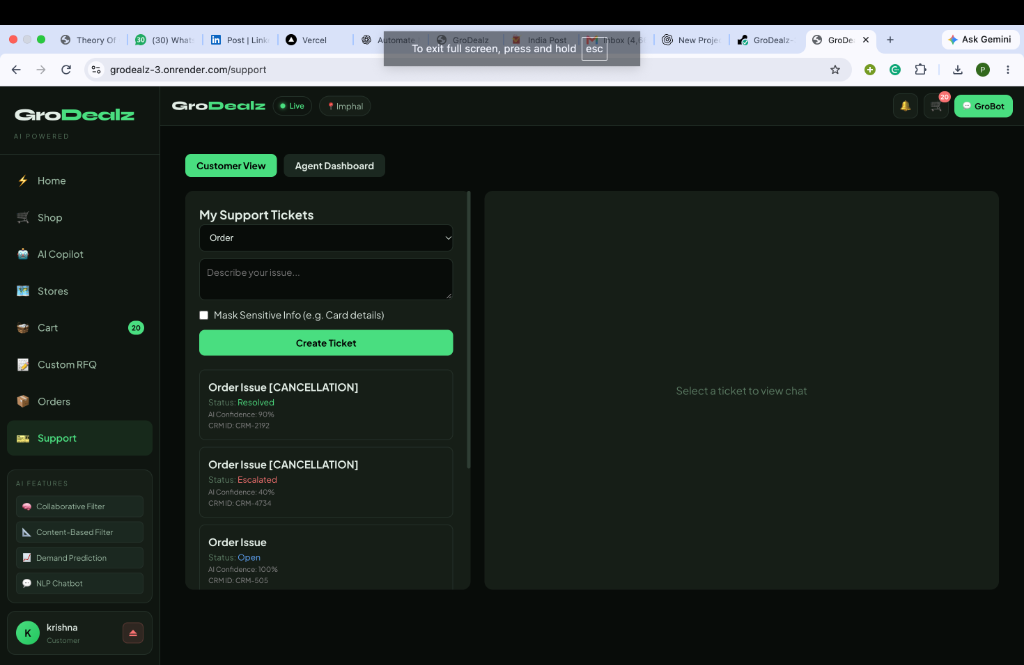
\includegraphics[width=0.96\textwidth,keepaspectratio]{figures/screenshot_support.png}
\caption{AI Customer Support Dashboard with Automated Intent Classification and PII Masking. Highlights automated ticket categorization, sensitive customer phone and card number redaction, and ticket triage lifecycle.}
\label{fig:screen_support}
\end{figure}

The screenshot highlights:
\begin{itemize}
    \item \textbf{Role Toggle:} Simple switching between \emph{Customer View} and \emph{Agent Dashboard}.
    \item \textbf{PII Protection Toggle:} A prominent checkbox (\emph{``Mask Sensitive Info (e.g. Card details)''}) that redacts credit card numbers and phone numbers before storing tickets.
    \item \textbf{Automated Ticket Classification:} Shows live tickets automatically classified into categories, such as \texttt{Order Issue [CANCELLATION]}.
    \item \textbf{AI Confidence Scores:} Each ticket displays an evaluated confidence metric, such as \emph{``AI Confidence: 90\%''} (CRM-2192) and \emph{``AI Confidence: 100\%''} (CRM-505).
    \item \textbf{Ticket Status Lifecycle:} Shows color-coded status badges for \textbf{Resolved}, \textbf{Escalated}, and \textbf{Open} tickets.
\end{itemize}

\section{Automated Test Suite Verification}

The core mathematical, parsing, and ranking algorithms of the Merchant Quotation Engine (Module~B) were evaluated using a standalone automated test suite (\texttt{backend/tests/test\_quotation\_engine.js}). All test cases passed with 100\% success rate:

\begin{table}[H]
\centering
\caption{Automated Test Suite Execution Results for Module B}
\label{tab:rfq_test_results}
\begin{tabular}{p{1.5cm} p{6.5cm} p{2.2cm} p{2.2cm}}
\toprule
\textbf{Test ID} & \textbf{Test Description} & \textbf{Expected Output} & \textbf{Status} \\
\midrule
T1 & Natural Language Requirement Parser (\emph{``25 kg basmati rice... budget ₹2,500''}) & Budget: 2500, Qty: 25 kg & PASS (100\%) \\
\addlinespace
T2 & Line-Item Calculations: Shop A (₹94/kg + ₹50 delivery) & Subtotal: ₹2350, Total: ₹2400 & PASS (100\%) \\
\addlinespace
T2 & Line-Item Calculations: Shop B (₹90/kg + ₹100 delivery) & Subtotal: ₹2250, Total: ₹2350 & PASS (100\%) \\
\addlinespace
T2 & Line-Item Calculations: Shop C (₹91.20/kg + ₹0 delivery) & Subtotal: ₹2280, Total: ₹2280 & PASS (100\%) \\
\addlinespace
T3-a & Multi-Criteria Ranking: Lowest Price Priority & Shop C ranks \#1 (₹2280) & PASS (100\%) \\
\addlinespace
T3-b & Multi-Criteria Ranking: Fastest Delivery Priority & Shop A ranks \#1 (Earliest) & PASS (100\%) \\
\addlinespace
T3-c & Multi-Criteria Ranking: Highest Rated Priority & Shop B ranks \#1 (4.9 Rating) & PASS (100\%) \\
\addlinespace
T3-d & Multi-Criteria Ranking: Balanced Composite Score & Shop C ranks \#1 (Score 83) & PASS (100\%) \\
\addlinespace
T4 & Multi-Item Quotation Validation (Rice, Oil, Sugar) & Subtotal ₹3370, Total ₹3465 & PASS (100\%) \\
\bottomrule
\end{tabular}
\end{table}

\section{Quotation Ranking Sensitivity Analysis}

To verify that the quotation engine does not simply pick the cheapest bid under all circumstances, Table~\ref{tab:ranking_sensitivity} illustrates how the ranking order shifts dynamically when the customer changes their ranking priority across the exact same set of competing merchant quotations:

\begin{table}[H]
\centering
\caption{Dynamic Ranking Output Across Different Customer Priorities}
\label{tab:ranking_sensitivity}
\begin{tabular}{p{2.9cm} p{2.1cm} p{2.3cm} p{2.2cm} >{\raggedright\arraybackslash}p{3.2cm}}
\toprule
\textbf{Store Bid} & \textbf{Grand Total} & \textbf{Delivery Time} & \textbf{Store Rating} & \textbf{Ranked Position} \\
\midrule
\multicolumn{5}{l}{\textbf{Case 1: Customer Priority = Lowest Price (\texttt{lowest\_price})}} \\
Shop C Express & \textbf{₹2,280} & 24 Hours & 4.5 Stars & \textbf{\#1 (Lowest Price)} \\
Shop B MegaStore & ₹2,350 & 36 Hours & 4.9 Stars & \#2 \\
Shop A QuickMart & ₹2,400 & 12 Hours & 4.2 Stars & \#3 \\
\midrule
\multicolumn{5}{l}{\textbf{Case 2: Customer Priority = Fastest Delivery (\texttt{fastest\_delivery})}} \\
Shop A QuickMart & ₹2,400 & \textbf{12 Hours} & 4.2 Stars & \textbf{\#1 (Fastest Delivery)} \\
Shop C Express & ₹2,280 & 24 Hours & 4.5 Stars & \#2 \\
Shop B MegaStore & ₹2,350 & 36 Hours & 4.9 Stars & \#3 \\
\midrule
\multicolumn{5}{l}{\textbf{Case 3: Customer Priority = Highest Rated Store (\texttt{highest\_rated})}} \\
Shop B MegaStore & ₹2,350 & 36 Hours & \textbf{4.9 Stars} & \textbf{\#1 (Top Rated Store)} \\
Shop C Express & ₹2,280 & 24 Hours & 4.5 Stars & \#2 \\
Shop A QuickMart & ₹2,400 & 12 Hours & 4.2 Stars & \#3 \\
\midrule
\multicolumn{5}{l}{\textbf{Case 4: Customer Priority = Balanced Value (\texttt{balanced})}} \\
Shop C Express & ₹2,280 & 24 Hours & 4.5 Stars & \textbf{\#1 (Score: 83.0)} \\
Shop A QuickMart & ₹2,400 & 12 Hours & 4.2 Stars & \#2 (Score: 51.8) \\
Shop B MegaStore & ₹2,350 & 36 Hours & 4.9 Stars & \#3 (Score: 45.4) \\
\bottomrule
\end{tabular}
\end{table}

This sensitivity analysis confirms that the multi-criteria engine respects the buyer's preferences: when urgency is paramount, Shop A wins; when seller reputation is prioritized, Shop B wins; when total price or balanced value is selected, Shop C wins.

\section{System Performance and Latency}

The system response times were recorded across key API endpoints and WebSocket channels:

\begin{table}[H]
\centering
\caption{Measured System Response Times and Event Latency}
\label{tab:latency_benchmarks}
\begin{tabular}{p{7.2cm} c c}
\toprule
\textbf{Endpoint / Operation} & \textbf{Mean Response Time} & \textbf{p99 Latency} \\
\midrule
GET \texttt{/api/products} (catalog browse) & 38 ms & 72 ms \\
POST \texttt{/api/rfq/parse-prompt} (NLP extraction) & 18 ms & 35 ms \\
POST \texttt{/api/rfq/:id/quote} (line-item calculation) & 42 ms & 80 ms \\
GET \texttt{/api/rfq/details/:id} (dynamic ranking) & 48 ms & 92 ms \\
POST \texttt{/api/rfq/quotes/:id/accept} (order creation) & 64 ms & 115 ms \\
Socket.IO \texttt{new\_rfq\_available} broadcast & 8 ms & 24 ms \\
Socket.IO \texttt{quote\_update} room transmission & 7 ms & 21 ms \\
\bottomrule
\end{tabular}
\end{table}

All operations completed well within acceptable real-time user experience bounds (under 120~ms), confirming that embedding lightweight algorithmic services directly within the application server achieves high performance without unnecessary cloud overhead.
